%! Author = lili
%! Date = 8/12/26

\section{Abgabe 1.6 \abhaken}\label{sec:abgabe-1.6}

\subsection{HA 1.6.1 \abhaken}\label{subsec:ha-1.6.1}
In einem Beutel liegen drei Münzen.
Wir wissen, dass zwei dieser Münzen fair sind, d.\,h., sie zeigen Kopf und Zahl mit derselben Wahrscheinlichkeit, wenn sie geworfen werden.
Die dritte Münze ist nicht fair und zeigt Kopf mit einer Wahrscheinlichkeit $p\ne \tfrac12$.

Wir wählen zufällig eine der Münzen, d.\,h., jede der Münzen wird mit derselben Wahrscheinlichkeit gewählt.
Im Anschluss werfen wir die gewählte Münze einmal.

\begin{auf}[(a) Geben Sie einen geeigneten Ereignisraum an, der es erlaubt, die folgenden Aufgabenteile zu bearbeiten.]
    $\ $
    \begin{figure}[H]
        \centering
        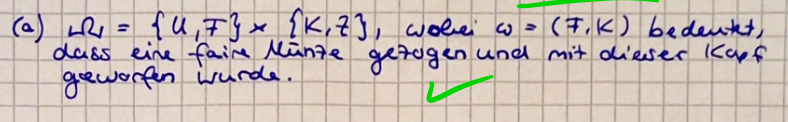
\includegraphics[width=0.8\linewidth]{images/lösungen/wts161a}\label{fig:figure38}
    \end{figure}
\end{auf}

\begin{auf}[(b) Definieren Sie die relevanten Ereignisse, und bestimmen Sie aus dem Text heraus deren Wahrscheinlichkeiten bzw.\ bedingte Wahrscheinlichkeiten.]
    $\ $
    \begin{figure}[H]
        \centering
        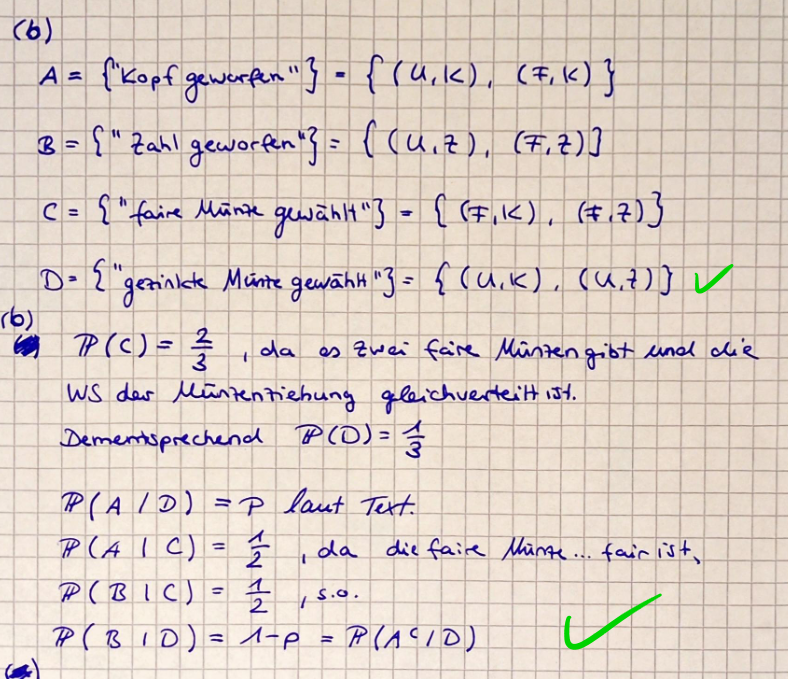
\includegraphics[width=0.8\linewidth]{images/lösungen/wts161b}\label{fig:figure37}
    \end{figure}
\end{auf}

\begin{auf}[(c) Berechnen Sie die Wahrscheinlichkeit, dass die gewählte Münze Kopf zeigt.]
    $\ $
    \begin{figure}[H]
        \centering
        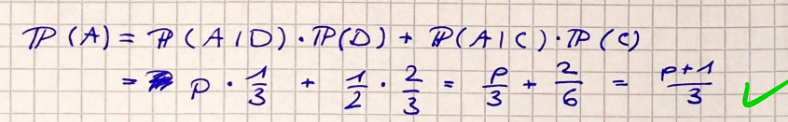
\includegraphics[width=0.8\linewidth]{images/lösungen/wts161c}\label{fig:figure36}
    \end{figure}
\end{auf}

\begin{auf}[(d) Berechnen Sie die bedingte Wahrscheinlichkeit, dass die gewählte Münze fair ist, gegeben, sie zeigt Kopf, nachdem wir sie, wie beschrieben, einmal geworfen haben.]
    $\ $
    \begin{figure}[H]
        \centering
        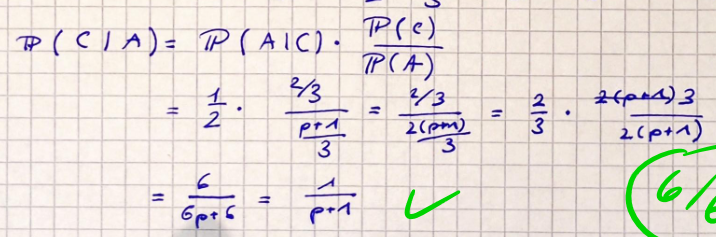
\includegraphics[width=0.8\linewidth]{images/lösungen/wts161d}\label{fig:figure35}
    \end{figure}
\end{auf}


\subsection{HA 1.6.2 \abhaken}\label{subsec:ha-1.6.2}
Beweisen Sie die Gedächtnislosigkeit der Exponentialverteilung, indem Sie zeigen, dass für jede exponentialverteilte Zufallsvariable (mit beliebigem Parameter)
\[
    P(X> t+s \mid X> s) = P(X> t) \qquad \forall\, s,t\ge 0
\]
gilt.

Was bedeutet dieses Resultat anschaulich, wenn Sie sich vorstellen, dass $X$ die Dauer eines langwierigen Telefongesprächs modelliert?

\begin{auf}[Lösung]
    $\ $
    \begin{figure}[H]
        \centering
        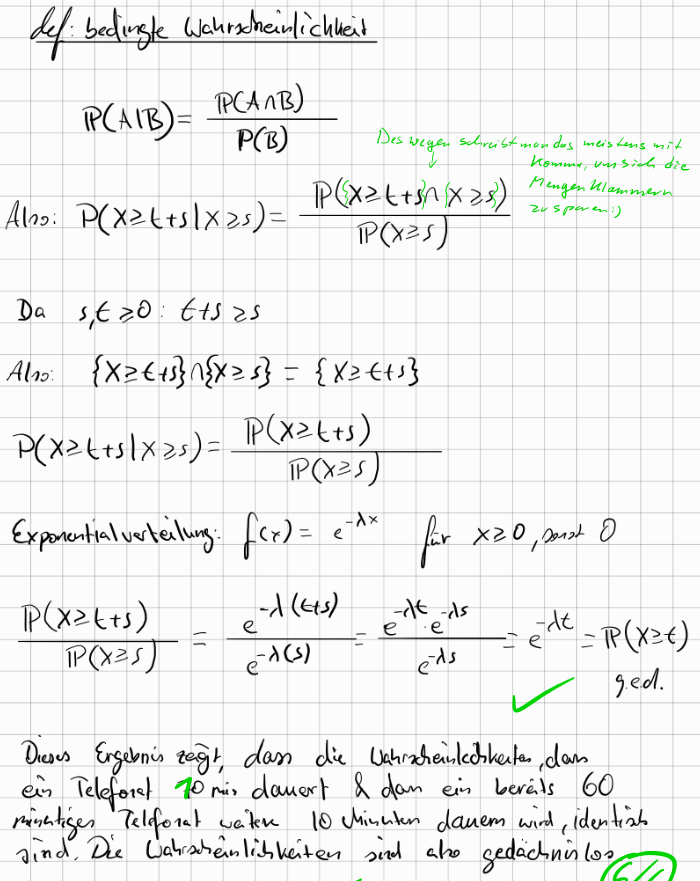
\includegraphics[width=0.8\linewidth]{images/lösungen/wts162}\label{fig:figure34}
    \end{figure}
\end{auf}

\subsection{HA 1.6.3 \abhaken}\label{subsec:ha-1.6.3}
Seien $(\Omega,\mu)$ ein Wahrscheinlichkeitsraum, $J$ eine abzählbare Indexmenge und $\{B_j\subseteq\Omega : j\in J\}$ eine Menge paarweise disjunkter Ereignisse mit $\Omega=\bigcup_{j\in J} B_j$.
Außerdem sei ein Ereignis $A\subseteq\Omega$ gegeben.

\begin{auf}[(a) Beweisen Sie den Satz von der totalen Wahrscheinlichkeit,]
    indem Sie zeigen:
    \[
        P(A) = \sum_{j\in J} P(A\mid B_j)\,P(B_j).
    \]
    \textit{Hinweis:} Sie können sich am Beweis des einfachsten Falls (siehe Vorlesung) orientieren.
    \begin{figure}[H]
        \centering
        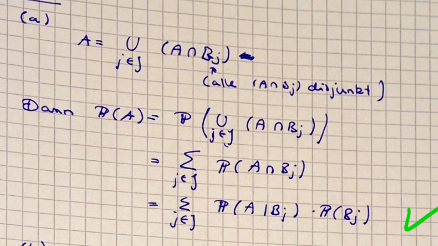
\includegraphics[width=0.8\linewidth]{images/lösungen/wts163a}\label{fig:figure33}
    \end{figure}
\end{auf}

\begin{auf}[(b) Es gelte zusätzlich, dass $P(A)>0$. Beweisen Sie die Bayes-Formel,]
    indem Sie für jeden Index $i$ zeigen:
    \[
        P(B_i\mid A) = \frac{P(A\mid B_i)\,P(B_i)}{\sum_{j\in J} P(A\mid B_j)\,P(B_j)}.
    \]
    \textit{Hinweis:} Sie dürfen die einfache Version der Bayes-Formel aus der Vorlesung sowie Aufgabenteil (a) verwenden.
    \begin{figure}[H]
        \centering
        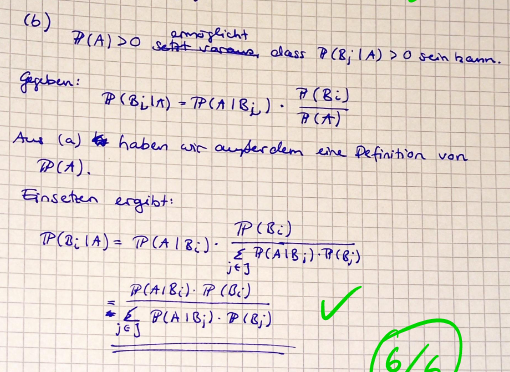
\includegraphics[width=0.8\linewidth]{images/lösungen/wts163b}\label{fig:figure32}
    \end{figure}
\end{auf}
